\section{Testing}
\subsection{Simulated Testbenches}
For the modules that were reused from exercise 1,
the associated testbenches were also reused.
When modules were modified,
so were the tests.

In addition to the provided processor testbench,
there are three separate testbenches created that each test the pipeline's ability to handle a specific hazard.
By making each of these tests pass, the provided testbench also started passing.

\begin{figure}[h]
    \centering
    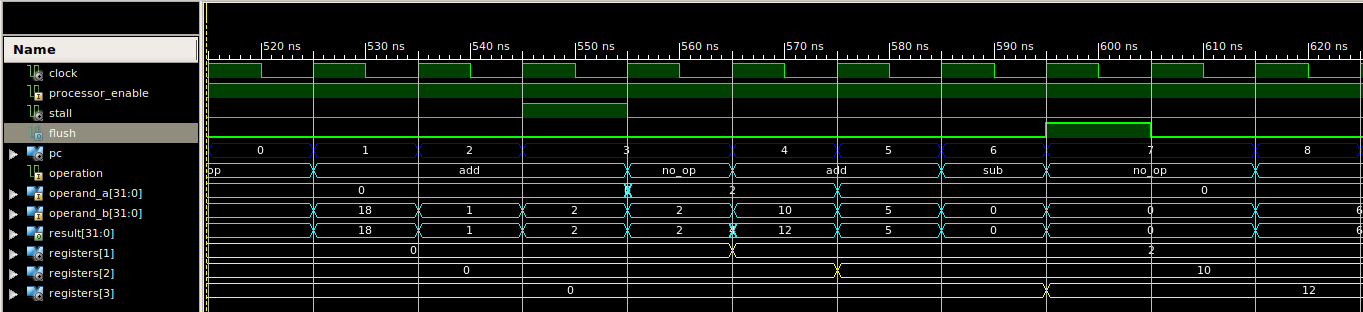
\includegraphics[width=\textwidth]{img/isim}
    \caption{Showing some assorted signals while \textit{ISim} simulates the provided testbench.\\
        The instruction \texttt{lw \$2, 2(\$0)} is fetched at PC=2 and is followed by \texttt{add \$3, \$1, \$2},
        requiring a stall.\\
        The add instruction can be seen executed at PC=4,
         and the resulting value 12 is written to register 3 by PC=7.
    }
    \label{fig:isim}
\end{figure}

\subsubsection{Forwarding Test}
Table \ref{tbl:forwarding} illustrates the pipeline executing the test program for the forwarding testbench.
RAW hazard are highlighted,
both where the EX stage needs forwarding to the ALU,
and where the ID stage needs register values before they are written.

\begin{table}[h]
    \begin{tabular}{l|lllll}
    ~  & IF                & ID                                  & EX                                                      & MEM                                   & WB \\ \hline
    0  & lw \$1, 1(\$0)    & ~                                   & ~                                                       & ~                                     & ~  \\
    1  & lw \$2, 2(\$0)    & lw \$1, 1(\$0)                      & ~                                                       & ~                                     & ~  \\
    2  & add \$3, \$1, \$1 & lw \$2, 2(\$0)                      & lw \$1, 1(\$0)                                          & ~                                     & ~  \\
    3  & add \$4, \$3, \$3 & add \$3, \$1, \$1                   & lw \$2, 2(\$0)                                          & lw \$1, 1(\$0)                        & ~  \\
    4  & sub \$5, \$4, \$3 & add \$4, \$3, \$3                   & add \$3, \textcolor{red}{\$1}, \textcolor{red}{\$1}     & lw \$2, 2(\$0)                        & lw \textcolor{red}{\$1}, 1(\$0)   \\
    5  & sw \$3, 3(\$0)    & sub \$5, \$4, \$3                   & add \$4, \textcolor{green}{\$3}, \textcolor{green}{\$3} & add \textcolor{green}{\$3}, \$1, \$1  & lw \$2, 2(\$0)   \\
    6  & sw \$4, 4(\$0)    & sw \textcolor{blue}{\$3}, 3(\$0)    & sub \$5, \textcolor{purple}{\$4}, \textcolor{blue}{\$3} & add \textcolor{purple}{\$4}, \$3, \$3 & add \textcolor{blue}{\$3}, \$1, \$1 \\
    7  & sw \$5, 5(\$0)    & sw \textcolor{brown}{\$4}, 4(\$0)   & sw \$3, 3(\$0)                                          & sub \$5, \$4, \$3                     & add \textcolor{brown}{\$4}, \$3, \$3 \\
    8  & ~                 & sw \textcolor{magenta}{\$5}, 5(\$0) & sw \$4, 4(\$0)                                          & sw \$3, 3(\$0)                        & sub \textcolor{magenta}{\$5}, \$4, \$3 \\
    9  & ~                 & ~                                   & sw \$5, 5(\$0)                                          & sw \$4, 4(\$0)                        & sw \$3, 3(\$0)   \\
    10 & ~                 & ~                                   & ~                                                       & sw \$5, 5(\$0)                        & sw \$4, 4(\$0)   \\
    11 & ~                 & ~                                   & ~                                                       & ~                                     & sw \$5, 5(\$0)   \\
    \end{tabular}
\caption{Pipeline containing RAW hazards}
\label{tbl:forwarding}
\end{table}

\subsubsection{Stalling Test}
Table \ref{tbl:stalling} shows the pipeline from the stalling testbench.
A value is being read to register 1, and is needed for the next instruction (addition).
Since the value won't be available until after the load instruction has passed the MEM stage,
the add instruction needs to be stalled.
Because forwarding has also been implemented, only one cycle of stalling is required.
\begin{table}[h]
    \begin{tabular}{l|lllll}
    PC & IF                & ID                & EX                & MEM               & WB                \\ \hline
    0  & lw \$1, 2(\$0)    & ~                 & ~                 & ~                 & ~                 \\
    1  & add \$1, \$1, \$1 & lw \$1, 2(\$0)    & ~                 & ~                 & ~                 \\
    2  & sw \$1, 3(\$0)    & add \$1, \$1, \$1 & lw \$1, 2(\$0)    & ~                 & ~                 \\
    2  & sw \$1, 3(\$0)    & add \$1, \$1, \$1 & ~                 & lw \$1, 2(\$0)    & ~                 \\
    3  & ~                 & sw \$1, 3(\$0)    & add \$1, \$1, \$1 & ~                 & lw \$1, 2(\$0)    \\
    4  & ~                 & ~                 & sw \$1, 3(\$0)    & add \$1, \$1, \$1 & ~                 \\
    5  & ~                 & ~                 & ~                 & sw \$1, 3(\$0)    & add \$1, \$1, \$1 \\
    6  & ~                 & ~                 & ~                 & ~                 & sw \$1, 3(\$0)    \\
    \end{tabular}
\caption{Pipeline containing structural hazards}
\label{tbl:stalling}
\end{table}

\subsubsection{Branching Test}
Table \ref{tbl:branching} shows the pipeline from the branching testbench.
In the test program a branch is taken which means the add instruction is not to be committed.
When the branch instruction reaches the MEM stage and updates the program counter,
the instructions from the wrong branch are flushed.

\begin{table}[h]
    \begin{tabular}{l|lllll}
    PC & IF                 & ID                 & EX                 & MEM              & WB               \\ \hline
    0  & lw   \$1, 1(\$0)   & ~                  & ~                  & ~                & ~                \\
    1  & beq  \$0, \$0, 1   & lw   \$1, 1(\$0)   & ~                  & ~                & ~                \\
    2  & add  \$2, \$1, \$1 & beq  \$0, \$0, 1   & lw   \$1, 1(\$0)   & ~                & ~                \\
    3  & no op (1)          & add  \$2, \$1, \$1 & beq  \$0, \$0, 1   & lw   \$1, 1(\$0) & ~                \\
    4  & no op (2)          & no op (1)          & add  \$2, \$1, \$1 & beq  \$0, \$0, 1 & lw   \$1, 1(\$0) \\
    3  & no op (1)          & (flushed)          & (flushed)          & (flushed)        & beq  \$0, \$0, 1 \\
    \end{tabular}
\caption{Pipeline containing a branch that is taken}
\label{tbl:branching}
\end{table}

\subsection{Testing on an FPGA}
The test program from exercise 1 was reused when implementing the new processor design on an FPGA.

\begin{figure}[h]
    \centering
    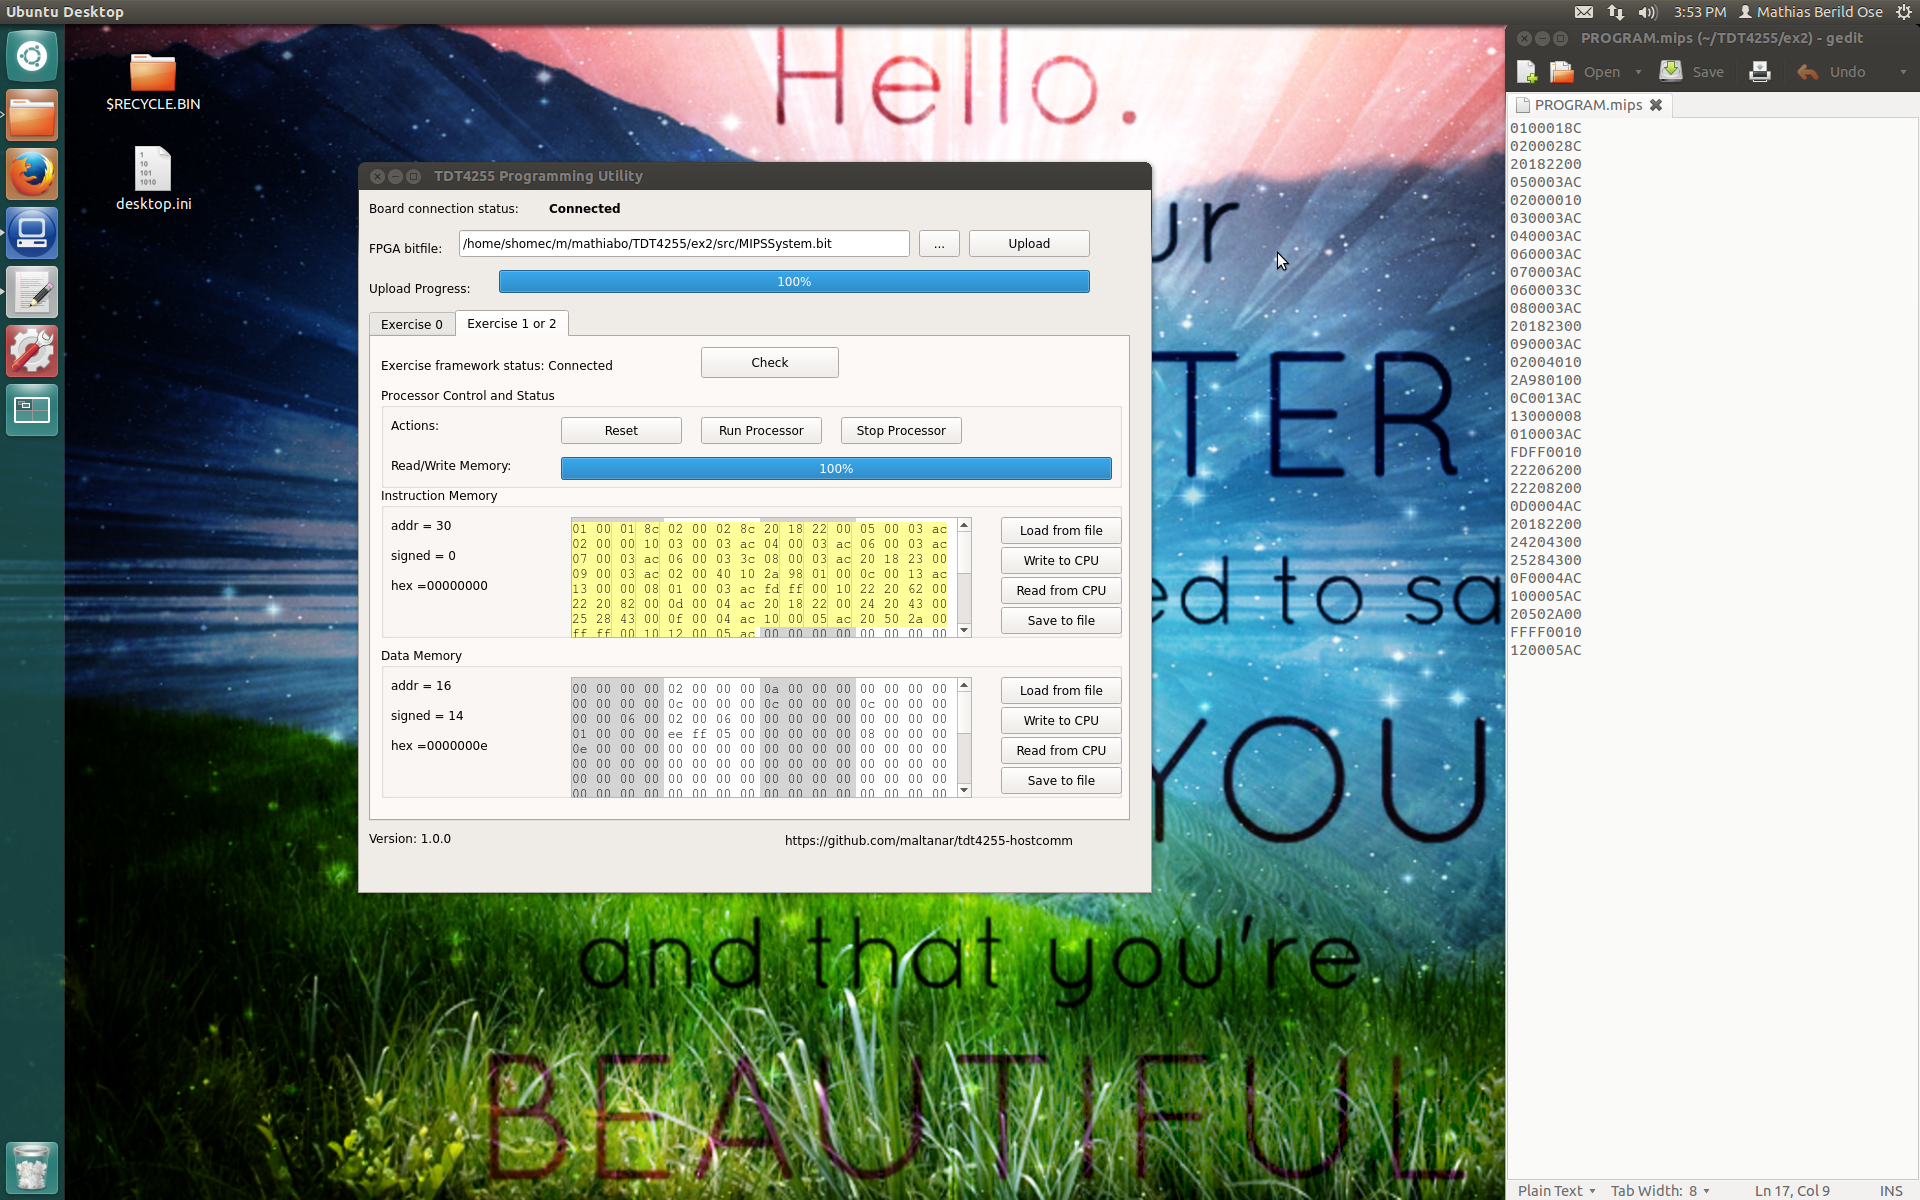
\includegraphics[width=\textwidth]{img/hostcomm}
    \caption{Resulting date memory loaded from FPGA after running the pipelined processor implementation with the test program.}
    \label{fig:hostcomm}
\end{figure}

